\documentclass{article}
\usepackage[utf8]{inputenc}
\usepackage{graphicx}
\usepackage{cite}
%Includes "References" in the table of contents
\usepackage[nottoc]{tocbibind}

\title{DL\_Project\_Contents}
\author{Lingfeng Zhang}
\date{December 2019}

\begin{document}

\maketitle

\section{Experiment Setup}

In this experiment, relationships between the existence of university perturbation and the dataset complexity, as well as the training model complexity should be found. There are three main steps to process experiments:

\begin{itemize}
    \item Generating images with different complexity levels
    \item Training models with different number of layers
    \item Generating the universal perturbation based on a certain complexity level dataset and a certain number of layers training model. 
\end{itemize}

\subsection{Generating images}

Some assumptions setting: 

images size and channel: 28*28*1

number of classes: 4

images number for each class: 1000

Firstly, 4 class baseline images should be created. See Figure~\ref{fig:baseline_image}.To generate these images, setting 1 as the pixel value on separated locations and uniform distribution random number ranged [0,1) on other unfilled locations. Making sure that the training model can recognise different class images. In this case, setting 1 on upper left corner 7*7 pixels and random number on other pixels represents class 0 images. And by the same logic, images of class 1, 2 and 3 are created. 
\begin{figure}[h]
    \centering
    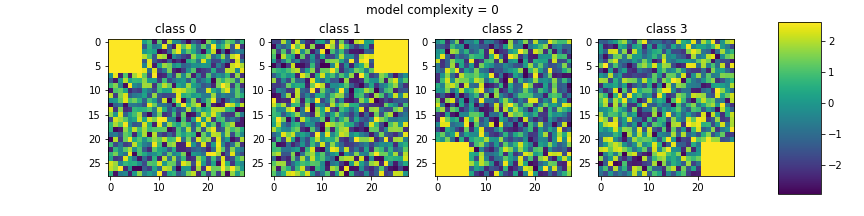
\includegraphics[width=1\linewidth]{demo-0.png}
    \caption{\small 4 class baseline images}
    \label{fig:baseline_image}
\end{figure}

While getting more complex dataset, more convolutional layers in the generating images model(called "images generator") should be added. The relation between them see formula (1). The weights and bias in convolutional layers do not need be learned in the images generator. These parameters are initialized and fixed by random values, uniform distribution random value for weights and normal distribution for bias.
\begin{equation}
    number\ of\ layers\ in\ generator\ \propto dataset\ complexity\ level
\end{equation}

After 2 layers convolutional computation, the baseline images are transferred into Figure~ \ref{fig:more_complex_image}. These images look like more complex than baseline images intuitively.
\begin{figure}[h]
    \centering
    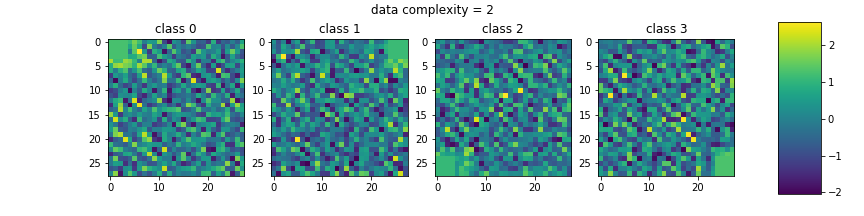
\includegraphics[width=1\linewidth]{demo-2.png}
    \caption{\small 4 class images after 2 convolutional computation}
    \label{fig:more_complex_image}
\end{figure}

It should be mentioned that all pixel values of one image will be close to a certain number(in most cases, close to 0) after original images passing the images generator with many convolutional layers. This is probably because feature boundaries of different class images fades with increasing times of convolutional computations. So, these images pixel values should be scaled. Feature boundary in this experiment is represented by the location of pixels with value 1.

There are several comments and tricks about the images generator model
\begin{itemize}
    
    \item To make sure that adding more layers in the images generator can get more complex dataset, weights in less layers of the images generator should be stored and used again on lower layers of the more layers images generator. Otherwise, if these weights are totally different random values, it will occur that the more layers generator may get lower complex dataset than the less layers generator. This is because all weights of the more layers generator are probably overall smaller than these weights of the less layers generator.
    
    \item This method to generate different complexity level dataset is reasonable because convolutional computation can gradually blur the decision boundary from baseline images dataset with increasing the convolutional layers.
    
    \item The number of convolutional layers in the images generator is in range from 0 to 9. When 10 convolutional layers are used in the generator, training model could not learn the decision boundary of these classes well, meaning testing accuracy is not good enough. This is probably because too many convolutional computations mix up the location information which can be recognised by the training model. In another word, too much layers in images generator will generate "garbage" images which can not be classified by training models well. After 9 layers convolutional computation, the baseline images are transferred into Figure~ \ref{fig:most_complex_image}. It is difficult to recognise which classes these images belong to by human eyes.
    
    \item To compare the size of universal perturbation generated from different complexity level dataset later, these images pixel values should be expanded or shrank to the same scale. So, these images pixels should be normalized after passing these convolutional layers.
    
    \item To avoid too much loss of baseline images' information, the activation function in each convolutional layers in images generator is LeakyRelu because other activation functions like ReLu, sigmoid, tanh or others, may induce values into saturation field, which cause the information loss.
    
    \item In the images generator, only convolutional layers are constructed because pooling layers may lead to the information loss from original images and dense layers may shuffle the location of representative pixels.
\end{itemize}

\begin{figure}[h]
    \centering
    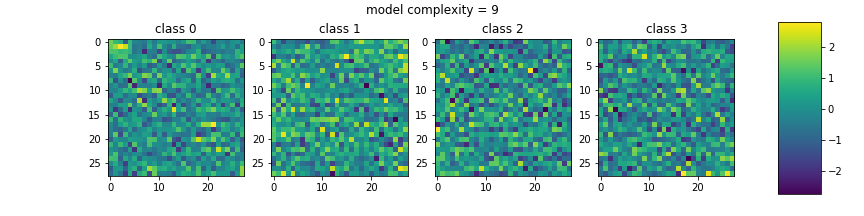
\includegraphics[width=1\linewidth]{demo-9.png}
    \caption{\small 4 class images after 9 convolutional computation}
    \label{fig:most_complex_image}
\end{figure}

The structure of images generator with 4 convolutional layers(dataset complexity level 4) is shown in Table ~\ref{table:generator_structure} and Figure ~\ref{fig:generator_structure}.

\begin{table}
\begin{center}
\begin{tabular}{ |c|c|c|c|c| } 
\hline
Height & Width & Depth & filter Height & filter Width \\
\hline
36 & 36 & 1 & 3 & 3 \\ 
\hline
34 & 34 & 32 & 3 & 3 \\ 
\hline
32 & 32 & 32 & 3 & 3 \\ 
\hline
30 & 30 & 32 & 3 & 3 \\ 
\hline
28 & 28 & 1 & None & None \\ 
\hline
\end{tabular}
\end{center}
\caption{The structure of images generator with 4 convolutional layers}
\label{table:generator_structure}
\end{table}

\begin{figure}[h]
    \centering
    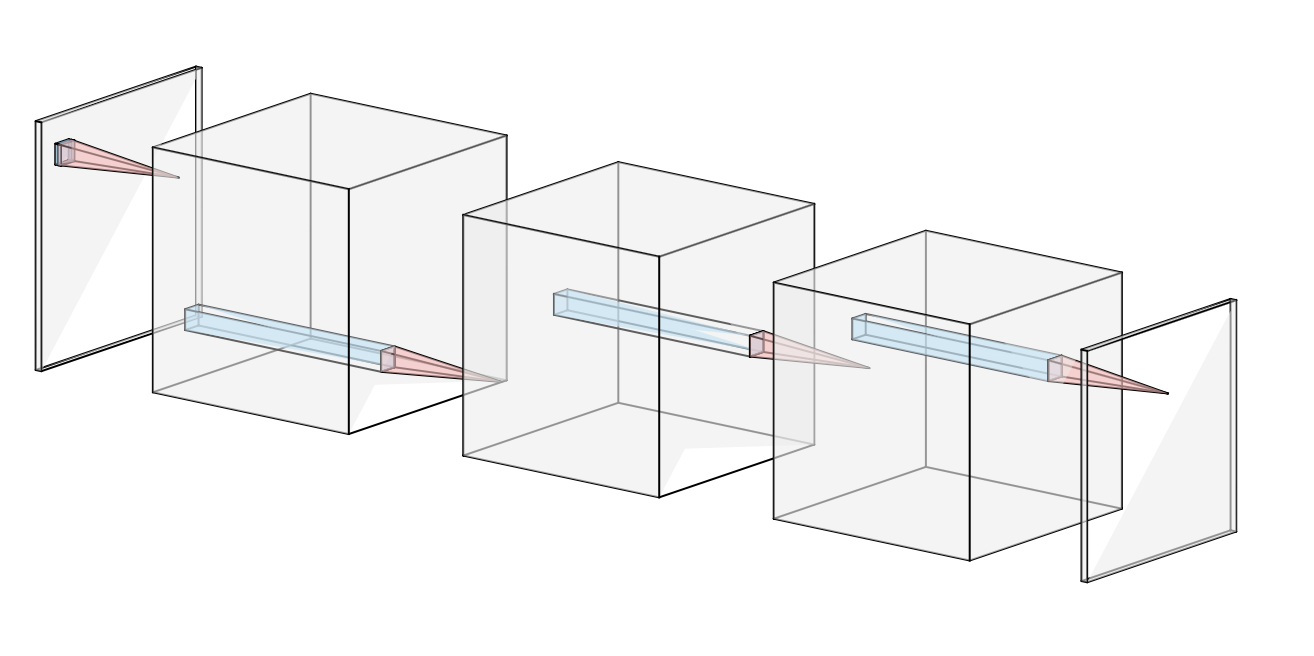
\includegraphics[width=1\linewidth]{generator_structure.png}
    \caption{\small The structure of images generator with 4 convolutional layers}
    \label{fig:generator_structure}
\end{figure}

To find the relation between the dataset complexity and the universal perturbation, the number of training model layers should be fixed on 4.
\subsection{Training models}

To get different complex training models, adding different number of layers can achieve this goal. Seven kinds of layers number are record: 3, 5, 8, 11, 14, 17 and 20. 3 layers training model includes 1 convolutional layer and 2 fully connected layers. Similarly, for 3, 5, 8 and 11 layers training models, they include 2 fully connected layers and \#layers-2 convolutional layers. With increasing too many convotional layers, the traning model can not perform well, but adding more fully connected layers based on sufficient number of convolutional layers can improve the training model performance again. So, for 14, 17 and 20 layers training models, they include 11 convolutional layers and \#layers-11 fully connected layers.

In addition, with increasing the number of layers in the training model, smaller learning rate should be applied because large learning rate could not help complex training models converge.

After fine tuning, all training models can reach up $99\%$ testing accuracy within small epochs. The activation function for all layers in all training models are ReLu. 

The structure of training model with 4 layers(2 convolutional layers and 2 dense layers) is shown in Table ~\ref{table:training_model_structure} and Figure ~\ref{fig:training_model_structure}.

\begin{table}
\begin{center}
\begin{tabular}{ |c|c|c|c|c|c| } 
\hline
Layer & Height & Width & Depth & filter Height & filter Width \\
\hline
Convolution & 28 & 28 & 1 & 3 & 3 \\ 
\hline
Convolution & 26 & 26 & 32 & 3 & 3 \\ 
\hline
Dense & 24 & 24 & 128 & None & None \\ 
\hline
Dense & 24 & 24 & 32 & None & None \\ 
\hline
Output & \multicolumn{2}{c}{4} & 1 & None & None \\ 
\hline
\end{tabular}
\end{center}
\caption{The structure of training model with 4 layers}
\label{table:training_model_structure}
\end{table}

\begin{figure}[h]
    \centering
    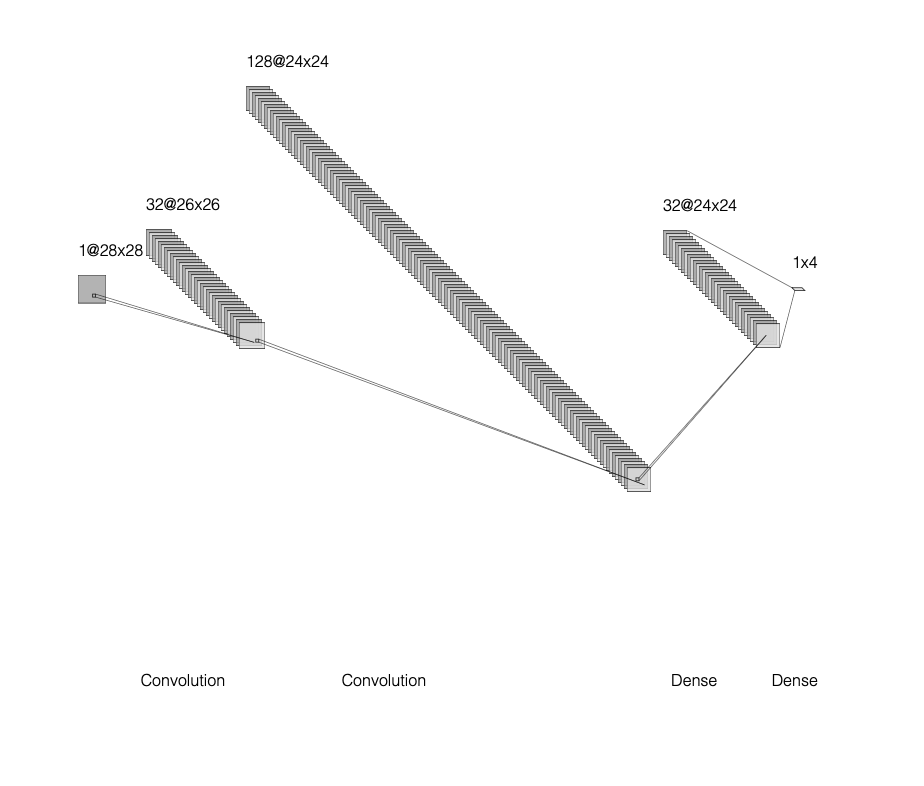
\includegraphics[width=1\linewidth]{training_model_structure.png}
    \caption{\small The structure of training model with 4 layers}
    \label{fig:training_model_structure}
\end{figure}

To find the relation between the training model complexity and the universal perturbation, the dataset complexity level(number of layers in images generator) should be fixed on 4.

\subsection{Generating the universal perturbation}

Some hyper-parameters setting
\begin{itemize}
    \item Images used to train the universal perturbation: 400 and 100 for each class
    \item Baseline Method to generate perturbation: Deep Fool
    \item Fooling rate $> 70\%$
    \item Metric to calculate the magnitude of universal perturbation: Infinity Norm $||\xi||_\infty$
    \item Maximum number of iterations to train the universal perturbation: 10
\end{itemize}

\section{Result Analysis}

\begin{table}
\begin{center}
\begin{tabular}{ |c|c|c| } 
\hline
Data complexity & Model layers & $\xi$ \\
\hline
0 & & 4.2 \\ 
1 & & 2.0 \\ 
2 & & 1.8 \\
3 & & 1.8 \\ 
4 & & 1.8 \\ 
5 & \multirow{4} & 1.6 \\ 
6 & & 1.6 \\ 
7 & & 1.6 \\ 
8 & & 1.1 \\ 
9 & & 0.9 \\ 
\hline
\end{tabular}
\end{center}
\caption{Relation between dataset complexity and universal perturbation}
\label{table:dc_up_table}
\end{table}

To visualize the Table \ref{table:dc_up_table}, see Figure~ \ref{fig:dc_up}.
\begin{figure}[h]
    \centering
    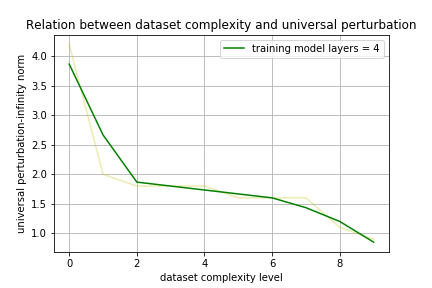
\includegraphics[width=1\linewidth]{dc_up.png}
    \caption{\small Relation between dataset complexity and universal perturbation}
    \label{fig:dc_up}
\end{figure}

The shallow line represents the original data points and solid line is the more smooth line generated from the shallow one by using Savitzky-Golay filter~\cite{LUO20051429}.

As shown in table, for example, when the data complexity is 0 and the number of training models layers is 4, if adding the universal perturbation is smaller than 4.2, then the fooling rate will less than $70\%$. The value of $\xi$ is the boundary to determine whether fooling rate is greater or smaller than $70\%$. So this value can show how easy the universal perturbation exists.

See Figure~ \ref{fig:per2}, when dataset complexity level is 1, adding universal perturbation with infinity norm 2.0 can fool training model to recognise one image of class 2 as class 3.
\begin{figure}[h]
    \centering
    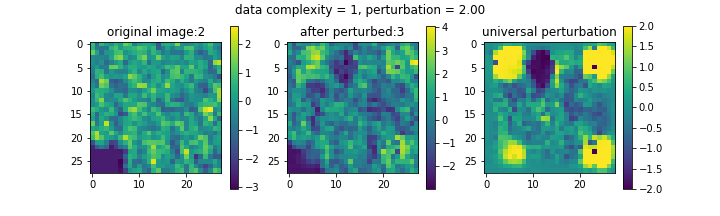
\includegraphics[width=1\linewidth]{model-c1-l4-pb-per2.png}
    \caption{\small Example of universal perturbation with infinity norm 2.0}
    \label{fig:per2}
\end{figure}

See Figure~ \ref{fig:per09}, when dataset complexity level is 9, adding universal perturbation with infinity norm 0.9 can fool training model to recognise one image of class 1 as class 3.
\begin{figure}[h]
    \centering
    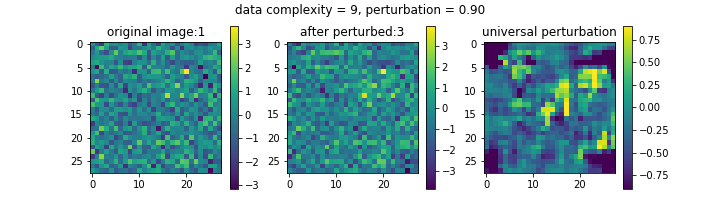
\includegraphics[width=1\linewidth]{model-c9-l4-pb-per09.png}
    \caption{\small Example of universal perturbation with infinity norm 0.9}
    \label{fig:per09}
\end{figure}

To compare these two universal perturbations, the universal perturbation with larger infinity norm changed the original images information more, like brute force  to change one class image to another class. This kind of universal perturbation is relatively meaningless than slight perturbation in real world.

When the dataset become more complex, smaller universal perturbation can be added on images to fool the training model well.

\begin{table}
\begin{center}
\begin{tabular}{ |c|c|c| } 
\hline
Model layers & Data Complexity & $\xi$ \\
\hline
3 & & 2.7 \\ 
5 & & 2.4 \\ 
8 & & 1.5 \\
11 & \multirow{4} & 1.5 \\ 
14 & & 1.3 \\ 
17 & & 1.2 \\ 
20 & & 1.5 \\ 
\hline
\end{tabular}
\end{center}
\caption{Relation between training model complexity and universal perturbation}
\label{table:tmc_up_table}
\end{table}

To visualize the Table \ref{table:tmc_up_table}, see Figure~ \ref{fig:tmc_up}.
\begin{figure}[h]
    \centering
    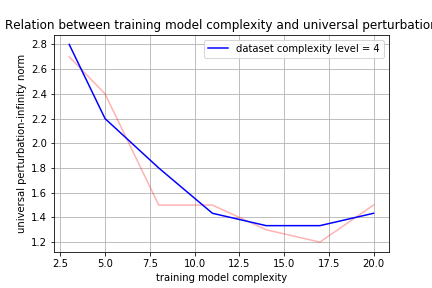
\includegraphics[width=1\linewidth]{tmc_up.png}
    \caption{\small Relation between training model complexity and universal perturbation}
    \label{fig:tmc_up}
\end{figure}

Overall, when the training model become more complex, smaller universal perturbation can be added on images to fool the training model well. In this experiment, the universal perturbation generated from 20 layers training model is slightly larger than those generated from 14 and 17 layers training models. This is probably because some bias of this experiment occur.

\section{Discussion and Future Work(addition)}
For the bias in the experiment, more experiments should be done to analyse why this noise happen. For example, adding more than 20 layers in training model to analyze the infinity norm of the universal perturbation.

In this experiment, adding more convolutional layers in images generator can control the complexity level of the datasets. But in real world, some methods should be found or applied to evaluate semantic datasets complexity, such as spectral metric~\cite{Branchaud-Charron_2019_CVPR} or other complexity measures.

Calculate the difference of different class images in various complexity level datasets by using Kullback–Leibler divergence of other metrics. Find whether the difference of different class images in complex datasets is smaller than that in simple datasets. 

Test the universality of universal perturbation and find whether there is a "global" universal perturbation. In this experiment, universal perturbation is "locally" universal, meaning it is a pattern can fool the training model trained on a certain dataset and may not fool the training model trained on other datasets in a high fooling rate.

\section{Conclusion(addition)}
To summarise, when the dataset and training model become more and more complex, the decision boundary gradually become unclear and difficult to be learnt by classifiers. So, there may exist an universal perturbation or a pattern to disturb original dataset information, inducing one class images can be added a small perturbation to "skip" into other decision areas.

\medskip

\bibliographystyle{unsrt}
\bibliography{reference}
\end{document}

